\documentclass[presentation]{beamer}

\usecolortheme{Imperial}
 
\usepackage[utf8]{inputenc}
\usepackage[UKenglish]{babel}
\usepackage{booktabs}
\usepackage{caption}
\usepackage{subcaption}
\usepackage{graphicx}
\usepackage{amsmath}
\usepackage{amsfonts}
\usepackage{amssymb}
\usepackage{epstopdf}
\usepackage{csquotes}
\usepackage{tikz}
\usepackage{media9}

% complying UK date format, i.e. 1 January 2001
\usepackage{datetime}
\let\dateUKenglish\relax
\newdateformat{dateUKenglish}{\THEDAY~\monthname[\THEMONTH] \THEYEAR}

% Imperial College Logo, not to be changed!
\institute{
\includegraphics[height=0.7cm]{Imperial_1_Pantone_solid.eps}}

\title{UROP 2023}

\author{Archibald Browne}

\begin{document}

\frame{\titlepage}

\begin{frame}{What did I do?}
    The project focused around formalising exercises from Professor M. Liebeck's 'A Concise Introduction to Mathematics' in Lean. Specifically, those from Chapter 10 'The Integers'.
    \pause
    \\ 
    \vspace{1em}
    The questions were mainly focused around the following areas:
    \begin{itemize}
        \item Greatest Common Divisor
        \item Lowest Common Multiple
        \item Bézout's Identity
        \item Prime Numbers
    \end{itemize}
    \pause
    I will go over some of the highlights/difficulties I experienced over the project, and what I learnt.
\end{frame}

% Question 8

\begin{frame}{Highlights}
    Here I will look at a couple of my favourite questions:
    \pause
    \begin{block}{Question 8}
        Let \(n \geq 2\) be an Integer. Prove that \(n\) is prime if and only if \(\forall a \in \mathbb{Z}, \  \gcd(a, n) = 1 \vee n \vert a \)
    \end{block}
    \pause
    \begin{itemize}
        \item Like many of the questions, this was much harder to teach to Lean than it was to solve. 
        \item The general idea is that prime numbers cannot have common factors with any numbers that aren't a multiple of that prime.
    \end{itemize}
\end{frame}

\begin{frame}{Highlights}
    Question Statement in Lean:
    \\
    \vspace{1em}
    
\includegraphics[width=\textwidth]{UROP presentation/Question8.png}
    \pause
    \\
    \vspace{1em}
    Lean is fussy about the distinction between integers and naturals, so even though we have declared \(2 \leq n\) and \(n \in \mathbb{Z}\), we still need to tell Lean that \(n\) is a natural number in order to use theorems about natural numbers.
    \\
    \vspace{1em}
    \pause
    For the \(\implies\) direction, we condition on whether \( n \vert a\). If it does, we get the result immediately. If not, then \(gcd(a, n) = 1\) because \( n\) is prime.
\end{frame}

\begin{frame}[fragile]{Highlights}
    For the \(\impliedby\) direction, we use the theorem:
    \begin{verbatim}
    Nat.prime_def_lt'
    \end{verbatim}
    Which says:
    \[n \in \mathbb{N} \text{ is prime} \iff \forall d \in (1, n) \cap \mathbb{N}, d \nmid n\]
    \pause
    We then condition over our assumption specialized for some particular \(d\) value:
    \begin{itemize}
        \item If \(gcd(d, n) = 1\) then clearly \(d \nmid n\)
        \item If \(n \vert d\) then we have \(d \geq n \), a contradiction.
    \end{itemize}
    
\end{frame}

% Question 9

\begin{frame}{Highlights}
    Another of my favourite questions was question 9:
    \begin{block}{Question 9}
        Let \(a, b\) be coprime integers. Prove that for any integer \(n\) there exists integers \(s, t\) with \(s > 0\) such that \(sa + tb = n\).
    \end{block}
    \pause
    The main steps are:
    \begin{itemize}
        \item By Bèzout, \( \exists s', t', s'a + t'b = 1\) since \(a, b\) are coprime
        \pause
        \item We don't know whether \( s' > 0 \), so we use a trick:
        \pause
        \item \((s' + kb)a + (t' - ka)b = 1) \ \forall k \in \mathbb{Z}\)
        \pause
        \item Increase \( k \) until \(s' + kb > 0\), multiply through by \(n\) and we get the result
    \end{itemize}

\end{frame}

\begin{frame}{Highlights}
    Question statement in lean:
    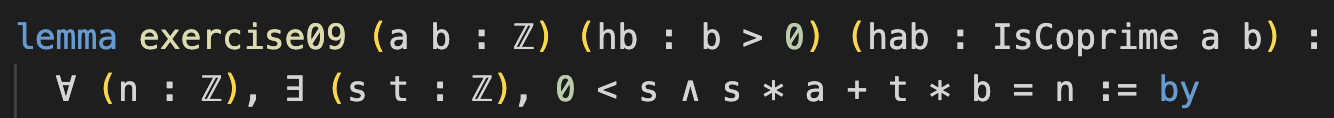
\includegraphics[width=\textwidth]{UROP presentation/Question9.png}
    \pause
    To help, I used the following helper lemma:
    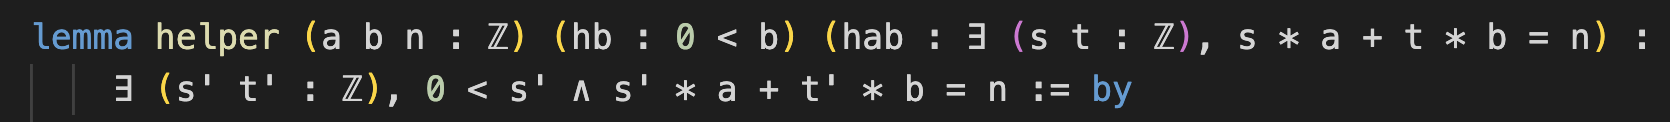
\includegraphics[width=\textwidth]{UROP presentation/Question9helper.png}
    This is the bulk of the question, and says that if we can find \(s, t\) with \(sa + tb = n\), then there is \(s', t'\) with \(s' > 0\) and \(s'a + t'b = n\).
\end{frame}

\begin{frame}{Highlights}
    The following two lines impliment the trick described on the earlier slide:
    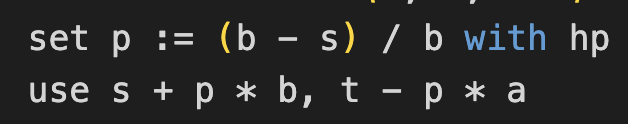
\includegraphics[width=\textwidth]{UROP presentation/Question9helperproof.png}
    \pause
    The rest of the proof of the helper proves that these are the correct choices of coefficients
\end{frame}



\begin{frame}{What did I Learn?}
    The project taught me quite a bit both about Lean, and undertaking a research project:
    \pause
    \begin{itemize}
        \item How to use Lean at a basic level
        \pause
        \item Developed interest in dependent type theory and functional programming (Curry-Howard Isomorphism etc.)
        \pause
        \item How to contribute to open source projects
    \end{itemize}
\end{frame}

\begin{frame}{What did I Learn?}
    I also learnt some more general things, unrelated to lean:
    \pause
    \begin{itemize}
        \item What it is like to work on a project (almost) by yourself
        \pause
        \item Acknowledging when you are stuck, and when to ask for help 
        \pause
        \item Informed my decision about whether to PhD or not 
    \end{itemize}
\end{frame}


\begin{frame}{Conclusion}
    Overall, huge thank you to Kevin for the opportunity, and everyone on the Xena discord for being so helpful!!!
    
\end{frame}
\end{document}